\section{АНАЛИТИЧЕСКИЙ ОБЗОР НАУЧНО-ТЕХНИЧЕСКОГО УРОВНЯ ПО ТЕМЕ ДИПЛОМНОГО ПРОЕКТА}
\label{sec:domain}

\subsection{Типовые схемы включения нелинейных регуляторов в системах управления мобильными роботами}
\label{sub:domain:1}
Рассмотрим типовую функциональную схему САУ [1]:

\begin{figure}[ht]
\centering
  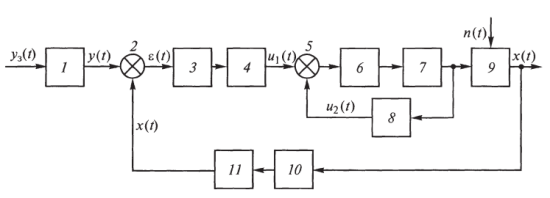
\includegraphics[scale=0.7]{1-1.png}  
  \caption{ Типовая функциональная схема САУ:
  1 – задающее устройство; 2, 5 – сравнивающие устройства; 3 – преобразующее устройство; 4, 8 – корректирующие устройства; 6 – усилительное устройство; 7 – исполнительное устройство; 9 – объект управления; 10 – измерительный элемент; элемент главной ОС.}
  \label{fig:domain:1:1}
\end{figure}

Задающее устройство 1 преобразует воздействие в сигнал, а сравнивающее устройство 2 в результате сравнения сигнала и регулируемой величины (предполагается, что элементы 10 и 11 не искажают сигнал) вырабатывает сигнал ошибки Сравнивающие устройства 2, 5 также называют датчиками ошибки, отклонения, рассогласования.

Преобразующее устройство 3 служит для преобразования одной физической величины в другую, более удобную для использования в процессе управления (во многих системах преобразующее устройство отсутствует).

Регуляторы 4, 8 служат для обеспечения заданных динамических свойств замкнутой системы. С их помощью обеспечивается высокая точность ее работы в установившемся режиме, а также демпфируются сильные колебательные процессы (например, летательных аппаратов). Более того, введение в систему регулятора позволяет устранить незатухающие или возрастающие колебания управляемой величины. Иногда регуляторы вырабатывают управляющие сигналы (команды) в зависимости от возмущающих воздействий, что существенно повышает качество работы систем, увеличивая их точность.

Из приведенной на рис. 1.1 схемы САУ видно, что в хорошо спроектированной системе ошибка очень мала, в то время как на управляемый объект должны поступать воздействия с мощностью, достаточной для питания двигателя. В связи с этим важным элементом САУ является усилительное устройство 6, предназначенное для повышения мощности сигнала ошибки, т.е. управления энергией, поступающей от постороннего источника. На практике широко используются электронные, магнитные, гидравлические и пневматические усилители.

Исполнительное устройство 7 предназначено для влияния на управляющий орган 9, подвергающийся воздействию внешних полей. Исполнительные устройства могут быть пневматические, гидравлические и электрические, которые подразделяются, в свою очередь, на электромоторные и электромагнитные.

Чувствительный (измерительный) элемент — датчик 10 — необходим в САУ для преобразования управляемых переменных в сигналы управления (например, угла в напряжение).

Элемент, который подвергается управлению, является объектом управления. При проектировании объектом управления считают всю неизменяемую часть САУ (т.е. все элементы, кроме регулятора). Это могут быть электрическая печь для закаливания металла, самолет, ракета, космический аппарат, двигатель, ядерный реактор, станок для обработки металла и т. д. В связи с большим разнообразием объектов управления разными могут быть и управляемые переменные: напряжение, число оборотов, угловое положение, курс, мощность и т.д.

\subsection{Виды нелинейных регуляторов}
\label{sub:domain:2}

Автоматический регулятор в системе регулирования состоит, как уже известно, из трех основных частей: измерительной, усилительно-преобразовательной и исполнительной. В усилительно-преобразовательной части имеются корректирующие устройства, в которых, помимо сигнала отклонения x регулируемой величины, образуется сигнал по первой производной. Закон, по которому формируется регулирующее воздействие и на объект из первичных сигналов называется законом регулирования. Математически закон регулирования определяется уравнением автоматического регулятора. Различают линейные и нелинейные законы регулирования.

Линейные законы регулирования определяются линейным уравнением регулятора и не рассматриваются в данной работе.

Что же касается нелинейных законов регулирования, то (за исключением релейного) они изучены мало. Очевидно, однако, что использование нелинейных законов регулирования, определяемых разнообразными нелинейными уравнениями регулятора значительно расширяет возможности целесообразного изменения качества процессов регулирования и точности. Это ясно из общих принципиальных соображений, так как область нелинейных уравнений значительно богаче и разнообразнее, чем линейных.

Введем следующую классификацию нелинейных законов регулирования [2]:

\begin{itemize}
  \item функциональные нелинейные законы регулирования,
  \item логические нелинейные законы регулирования,
  \item оптимизирующие нелинейные законы регулирования,
  \item параметрические нелинейные законы регулирования.
\end{itemize}

Важным отличием нелинейных законов от линейных является то, что они придают системе регулирования принципиально новые свойства. Если при линейном законе всегда вырабатывается сигнал, пропорциональный входной переменной или ее производной и т. д., то при нелинейном законе может существенно изменяться сам характер действия системы управления на объект в зависимости от величины входного воздействия. Другими словами, если для линейных систем изменение размера отклонения — это изменение только масштаба, но не формы процессов, то в нелинейной системе при этом может существенно изменяться и форма процессов, вплоть до принципиальных качественных изменений картины процессов. Эти особые свойства нелинейных законов можно выгодно использовать в технике автоматического управления и регулирования.

Рассмотрим отдельно каждый из указанных четырех классов нелинейных законов регулирования.

\textit{Функциональные нелинейные законы регулирования}. Функциональными будем называть такие нелинейные законы регулирования, при которых регулирующее воздействие на объект выражается в виде нелинейной функции от отклонения регулируемой величины, представляющей собой входную информацию для системы регулирования.

Данный класс может содержать в себе как статические, так и динамические нелинейности. 

В отличие от линейного закона, здесь в первом случае будет более энергичное действие регулятора при больших отклонениях х и большой запас устойчивости установившегося режима. Во втором случае будет менее энергичное, но более плавное действие регулятора вначале и повышенная точность в установившемся режиме, хотя и с меньшим запасом устойчивости. Однако такого рода рекомендации, как увидим в дальнейшем, справедливы для большинства систем, но все же не для всех. Поэтому они требуют специального обследования для каждого объекта регулирования.

Нелинейный закон регулирования за счет дополнительных нелинейных обратных связей может включать в себя также нелинейности от выходной величины, что расширяет возможности целесообразного изменения качества процесса регулирования.

Отметим, что функциональные нелинейные законы регулирования могут быть связаны не только с изменением параметров в зависимости от размеров входных воздействий, но и с изменением структуры. Например, при увеличении отклонения регулируемой величины сверх определенного порога в системе может происходить переключение с одного линейного корректирующего устройства на другое.

\textit{Логические нелинейные законы регулирования}. Нелинейные законы регулирования могут иметь иные формы, которые реализуются с помощью не функциональных, а более или менее сложных логических устройств. Будем называть их логическими нелинейными законами регулирования [2].

Логические нелинейные законы регулирования могут быть связаны также с изменением структуры системы регулирования. Например, при помощи логического устройства можно включать и выключать сигналы управления по первой и второй производным и по интегралу, в зависимости от сочетания значений отклонения регулируемой величины х и скорости отклонения. Если правильно сформировать логику этих переключений, то можно существенно повысить качество работы системы регулирования.

Вместо комбинирования указанных линейных членов закона регулирования могут вводиться также и функциональные нелинейные члены; включение и выключение сигналов, соответствующих этим членам, производится при помощи логического устройства. Тогда получится комбинация функциональных и логических нелинейных законов регулирования.

\textit{Оптимизирующие нелинейные законы регулирования}. В настоящее время интенсивно развивается теория оптимальных процессов регулирования. При этом на основе классических вариационных методов, или на основе так называемого принципа максимума, или методом динамического программирования определяется закон регулирования таким образом, чтобы система имела максимум быстродействия, или минимум ошибки, или же минимум какой-нибудь другой величины (в форме функционала) с учетом ограничений, накладываемых в реальной системе на координаты, скорости, силы и т. д. Как правило, при этом приходят к нелинейным законам регулирования, хотя, вообще говоря, можно оптимизировать и коэффициенты линейного закона, задав его форму. Часто оптимальный нелинейный закон регулирования состоит в переключении управляющего воздействия (при определенных состояниях системы) с одного максимально возможного значения на другое (противоположного знака). Моменты переключения в целом определяются сложными комбинациями значений нескольких переменных и их производных.

\textit{Параметрические нелинейные законы регулирования}. В предыдущих типах законов регулирования вводились отклонения регулируемой величины от некоторых заданных ее программных значений. При параметрической программе управления закон регулирования может выражаться в виде нелинейной функции текущих координат, в которых задается параметрическая программа.

Нелинейные законы регулирования обладают богатыми возможностями во всех случаях, когда требуемый эффект может быть достигнут изменением свойств системы с изменением величин ошибок. Важным классом нелинейных систем являются системы с переменной структурой. Большими возможностями обладают так называемые адаптивные, т. е. самонастраивающиеся и самоорганизующиеся, системы, примером которых служат алгоритмы нечеткой логики.

\subsection{Классические алгоритмы нечеткого вывода.  Мамдани и Сугено Тагаки}
\label{sub:domain:3}


\textit{Алгоритм Мамдани }(Mamdani) нашел применение в первых нечетких системах автоматического управления. Был предложен в 1975 году английским математиком Е. Мамдани для управления паровым двигателем [3].

Формирование базы правил системы нечеткого вывода осуществляется в виде упорядоченного согласованного списка нечетких продукционных правил в виде «IF A THEN B», где антецеденты ядер правил нечеткой продукции построены при помощи логических связок «И», а консеквенты ядер правил нечеткой продукции простые.

Фаззификация входных переменных осуществляется описанным выше способом, так же, как и в общем случае построения системы нечеткого вывода.

Агрегирование подусловий правил нечеткой продукции осуществляется при помощи классической нечеткой логической операции «И» двух элементарных высказываний A, B.

Активизация подзаключений правил нечеткой продукции осуществляется методом min-активизации, где $\mu (x)$ и c – соответственно функции принадлежности термов лингвистических переменных и степени истинности нечетких высказываний, образующих соответствующие следствия (консеквенты) ядер нечетких продукционных правил.

Аккумуляция подзаключений правил нечеткой продукции проводится при помощи классического для нечеткой логики max-объединения функций принадлежности.

Дефаззификация проводится методом центра тяжести или центра площади.

\textit{Алгоритм Сугено (Sugeno)} выглядит следующим образом [3]:

Формирование базы правил системы нечеткого вывода осуществляется в виде упорядоченного согласованного списка нечетких продукционных правил в виде «IF A AND B THEN $w=\epsilon_1 a + \epsilon_2 b $», где антецеденты ядер правил нечеткой продукции построены из двух простых нечетких высказываний A, B при помощи логических связок «И», a и b – четкие значения входных переменных, соответствующие высказываниям A и B , $\epsilon_1$ и $\epsilon_2$ – весовые коэффициенты, определяющие коэффициенты пропорциональности между четкими значениями входных переменных и выходной переменной системы нечеткого вывода, w – четкое значение выходной переменной, определенное как действительное число.

Фаззификация входных переменных, определяющих высказывания и осуществляется аналогично алгоритму Мамдани.

Агрегирование подусловий правил нечеткой продукции осуществляется аналогично алгоритму Мамдани при помощи классической нечеткой логической операции «И» двух элементарных высказываний A, B.

Активизация подзаключений правил нечеткой продукции проводится в два этапа. На первом этапе, степени истинности c заключений (консеквентов) нечетких продукционных правил, ставящих в соответствие выходной переменной действительные числа, находятся аналогично алгоритму Мамдани, как алгебраическое произведение весового коэффициента и степени истинности антецедента данного нечеткого продукционного правила. На втором этапе, в отличие от алгоритма Мамдани, для каждого из продукционных правил вместо построения функций принадлежности подзаключений в явном виде находится четкое значение выходной переменной $w= \epsilon_1 a+ \epsilon_2 b$ . Таким образом, каждому i-му продукционному правилу ставится в соответствие точка ( $c_i; w_i$ ) , где $c_i$ – степень истинности продукционного правила, $w_i$ – четкое значение выходной переменной, определенной в консеквенте продукционного правила.

Аккумуляция заключений правил нечеткой продукции не проводится, поскольку на этапе активизации уже получены дискретные множества четких значений для каждой из выходных лингвистических переменных.

Дефаззификация проводится как и в алгоритме Цукамото. Для каждой лингвистической переменной осуществляется переход от дискретного множества четких значений $\{w_1...w_n\}$ к единственному четкому значению согласно дискретному аналогу метода центра тяжести.


\subsection{Проблема разработки, тестирования и отладки алгоритмов управления}
\label{sec:domain:4}

Создание современных АСУ требует дальнейшего повышения качества управления за счет использования высокоэффективных алгоритмов управления. Использование таких алгоритмов сдерживалось их сложностью и аналоговой элементной базой. Даже широкомасштабный процесс перехода на цифровую элементную базу не обеспечил соответствующего повышения качества управления из-за трудностей при реализации режима жесткого реального времени. Вторым сдерживающим фактором являлась высокая трудоемкость разработки программного обеспечения (ПО) АСУ.

Для экономии времени и ресурсов при разработке роботов используются симуляторы. Симулятор создает программную модель робота и его окружения и имитирует его поведение в соответствие с программой. Симулятор позволяет создавать ПО в независимости от физической реализации робота и изменять модель робота без физических модификаций. В некоторых случаях программы, созданные для работы с моделью в симуляторе, могут быть перенесены на робота без изменений.

Среди новейших технологий, доступных сегодня для программирования, являются те, которые используют виртуальную симуляцию. Написание кода для моделирования также проще, чем писать код для физического робота. Хотя переход к виртуальным симуляциям для программирования роботов является шагом вперед в дизайне пользовательского интерфейса, многие такие приложения находятся только в зачаточном состоянии.



